\documentclass[11pt]{article}

% Change "review" to "final" for camera-ready or "preprint" for a non-anonymous version.
\usepackage[final]{acl}

\usepackage{times}
\usepackage{latexsym}
\usepackage[T1]{fontenc}
\usepackage[utf8]{inputenc}
\usepackage{microtype}
\usepackage{inconsolata}
\usepackage{graphicx}
\usepackage{booktabs}
\usepackage{tabularx}
\usepackage{array}
\usepackage{enumitem}
\usepackage{url}
\usepackage{amsmath}
\usepackage{amssymb}
\usepackage{pgfplots}
\pgfplotsset{compat=1.18}

\newcommand{\model}[1]{\textsc{#1}}
\newcommand{\tool}[1]{\texttt{#1}}
\newcommand{\dataset}[1]{\textsc{#1}}
\newcommand{\metric}[1]{\textsc{#1}}
\newcommand{\ours}{Nano-MemGPT}

\setlength{\tabcolsep}{4pt}

\title{
Diagnosing Small-Model Failures in MemGPT-Style Memory Retrieval\\
\large Tool-Call Control, Query Policy, and Teacher-Trajectory Distillation
}

\author{
Hyogi Kim\\
Ulsan National Institute of Science and Technology\\
\texttt{jeff4380@unist.ac.kr}
}

\begin{document}
\maketitle

\begin{abstract}
MemGPT-style agents turn long-term recall into a control problem: the model must decide when to search, what to search for, how to read the evidence it gets back, and when to answer. We study this loop on MSC Deep Memory Retrieval with Llama-3-8B and Mistral-7B, and find that small models fail it in stages rather than all at once. In a vanilla Letta/MemGPT setup neither model even satisfies the tool-call contract, so retrieval cannot yet be scored; a strict formatting adapter restores the loop but leaves containment at $0.1954$. To localize the remaining loss, we distill audited GPT-4.1 trajectories into the student and probe the loop one component at a time. On matched rows the distilled adapter climbs from $0.5797$ to $0.8668$ judge accuracy when handed the teacher's retrieved evidence, but only to $0.6294$ when given its query strings---so the binding constraint is acquiring evidence, not generating answers, with query selection a real yet partial part of it. Small hard-set SFT and DPO do not generalize, whereas a non-oracle retrieval-feedback reranker recovers the reference in $25/72$ teacher-only hard cases. We argue that small memory agents should be evaluated component by component, keeping query policy and evidence handling distinct from end-to-end accuracy.
\end{abstract}

\section{Introduction}

Conversational agents that persist across sessions must answer questions whose evidence is no longer in the active context. A user may later ask, ``Where did I say I work on weekends?'' or ``What artist did I say I could get into?'' Such questions are not tests of world knowledge alone; they require recovering a particular prior utterance and grounding the answer in it.

MemGPT-style systems address this setting by treating the language model as a controller over memory tools. Instead of answering immediately, the model may call \tool{conversation\_search}, inspect retrieved messages, issue additional searches, and then answer. This design is attractive because it separates a limited context window from a larger external memory. It also introduces a less visible source of difficulty: the model must decide how to operate the memory system.

End-to-end DMR accuracy therefore conflates several distinct abilities. A wrong answer might mean the model never emitted a valid tool call, or searched for a paraphrase the substring retriever could not match, or retrieved the right memory and then ignored it, or buried it among distractors. We study these failure modes directly, on Llama-3-8B and Mistral-7B in a local Letta/MemGPT setup on MSC Deep Memory Retrieval (DMR), asking how much of the loss belongs to tool-channel control, query policy, evidence acquisition, and answer grounding.

Rather than propose a new memory architecture, we treat the loop itself as the object of measurement. Small models, it turns out, can fail before retrieval even begins; teacher evidence can mask a weak search policy; and trajectory distillation stabilizes the loop without teaching the literal queries the local retriever rewards. We therefore report tool transport, query policy, retrieval feedback, evidence filtering, and answering as separate error sources before recombining them in the full agent.

\section{Background and Related Work}

\paragraph{Memory-augmented LLM agents.}
MemGPT introduced virtual context management for LLMs, drawing an analogy to operating systems that move information between fast and slow memory tiers \citep{packer2023memgpt}. In multi-session chat, the model can query recall memory to retrieve previous dialogue. Later memory systems explore structured memory architectures: Zep/Graphiti uses temporal knowledge graphs for agent memory \citep{rasmussen2025zep}, while Memory-R1 studies reinforcement learning for memory operations \citep{yan2025memoryr1}. All three frame memory as an active control problem, but none isolates where a small model breaks down inside a Letta/MemGPT DMR loop.

\paragraph{Long-term conversational memory benchmarks.}
DMR evaluates whether an agent can recover personal facts from multi-session chat. The original MemGPT evaluation showed that recall memory improves over fixed-summary baselines \citep{packer2023memgpt}. More recent work reports high DMR scores for GPT-4-class or GPT-4o-mini-class systems, suggesting that DMR may be relatively easy for large modern models when full conversation or a strong memory layer is available \citep{rasmussen2025zep}. LongMemEval \citep{wu2024longmemeval} and LoCoMo \citep{maharana2024locomo} stress longer and more diverse memory behavior. In contrast, our experiments isolate the control interface used by smaller open-source models inside a MemGPT-style DMR loop.

\paragraph{Tool use, distillation, and query policy.}
Distilling a stronger model's trajectories into a smaller one is the natural recipe, and we follow it with Low-Rank Adaptation (LoRA) \citep{hu2021lora} alongside a small Direct Preference Optimization (DPO) pilot \citep{rafailov2023dpo}. The catch is that a trajectory folds four things together---tool-call formatting, search-phase query generation, the decision to stop and answer, and final answer grounding---so lowering token-level loss need not improve the query policy that actually controls retrieval. We therefore treat query policy as a separate object of study: under substring recall, a useful query is a literal phrase likely to appear in past dialogue, not a semantic summary of the question.

\section{Task, Models, and Evaluation}

\subsection{Deep Memory Retrieval}

Each DMR row contains previous multi-session dialogue, a current user probe, and a reference answer. The probe often asks indirectly about a previously stated personal fact, so the answer is usually not recoverable from the probe alone. For example:
\begin{quote}\small
\textbf{Probe:} Hey, remember that time we talked about music? What was the artist you mentioned you could get into?\\
\textbf{Reference:} Taylor Swift!
\end{quote}
The answer-bearing memory may be a previous utterance such as ``A little bit. I can get into Taylor Swift.'' In our Letta/MemGPT setup, each row creates a fresh agent, captures previous dialogue into recall storage, removes those messages from immediate context, and sends only the probe. This forces the model to use memory tools rather than simply reading the full dialogue in context.

\subsection{Local Substring Recall Contract}

Pilot experiments revealed a mismatch between maintained Letta tool descriptions and the local retrieval path. The maintained tool description suggested semantic/hybrid retrieval, while the local PostgreSQL recall path used case-insensitive substring matching. We therefore define a local \emph{substring recall contract}:
\begin{quote}\small
\tool{conversation\_search(query)} returns previous messages whose content contains \tool{query} under case-insensitive substring matching.
\end{quote}
This contract makes query formulation critical. A semantic query such as \tool{audio studio location} may fail if that phrase never appears in memory, while shorter literal anchors such as \tool{studio}, \tool{California}, or \tool{Santa Barbara} can succeed.

\subsection{Models and Metrics}

We evaluate \model{Llama-3-8B} \citep{grattafiori2024llama3} (\tool{NousResearch/Meta-Llama-3-8B-Instruct}) as the main student and LoRA target, \model{Mistral-7B} \citep{jiang2023mistral} (\tool{mistralai/Mistral-7B-Instruct-v0.3}) as a frozen replay comparison, and \model{GPT-4.1} (\tool{gpt-4.1-2025-04-14}) as teacher and judge. Local 7B/8B experiments use BF16 serving without quantization. We use LoRA rather than full fine-tuning due to GPU memory constraints.

We report loop completion, format failure, search rate, retrieved-reference, containment, ROUGE-L recall \citep{lin2004rouge}, and GPT-4.1 judge accuracy. Retrieved-reference means that at least one retrieved memory contains the reference answer under the same strict matching used for containment. Containment is strict and can reject valid paraphrases; judge accuracy can accept paraphrases but may be lenient. We therefore use both and audit their disagreement for teacher data.

\section{Method}

We run a sequence of controlled interventions, each removing or repairing one part of the loop so that whatever fails next can be read more narrowly. Table~\ref{tab:ladder} lays out the ladder.

\begin{table*}[t]
\centering
\small
\begin{tabularx}{\textwidth}{l X X}
\toprule
\textbf{Stage} & \textbf{Question} & \textbf{Diagnostic} \\
\midrule
Vanilla MemGPT & Can the small model enter the tool loop? & Raw Letta/MemGPT DMR \\
Strict template & Is the first barrier only tool-call surface form? & Rule-based parser/template repair \\
Full history & Can the model answer when search is removed? & Full previous dialogue in prompt \\
Teacher trace replay & Can the model answer with teacher evidence? & Replay approved GPT-4.1 tool outputs \\
LoRA distillation & Can teacher trajectories teach the loop? & Full trajectory LoRA r8/r16 \\
Teacher query hint & How much does better query selection help? & Teacher query chain + student execution \\
Query-only LoRA & Can query policy be learned separately? & Search-call-only SFT \\
Deterministic skeleton & What if the model only emits query strings? & Fixed tool wrapper \\
Teacher query replay & How far is student query quality from teacher query quality? & Replay teacher query strings \\
Hard SFT/DPO & Can hard examples repair the gap? & Positive SFT and zero-result DPO \\
Candidate reranking & Can retrieval feedback help at search time? & Generate multiple queries and rerank \\
Evidence filtering & Can answer context be reduced? & Non-oracle top-$k$ evidence filter \\
\bottomrule
\end{tabularx}
\caption{Controlled interventions used to decompose small-model MemGPT failure.}
\label{tab:ladder}
\end{table*}

\section{Results}

\subsection{Raw Small Models Fail the Tool-Call Contract}

In a raw vanilla Letta/MemGPT pilot, Llama-3-8B and Mistral-7B both fail all five DMR rows before retrieval quality is ever in question. The result says nothing about retrieval; it says that an untrained small instruction model does not reliably satisfy the structured tool-call contract.

\begin{table}[t]
\centering
\small
\begin{tabular}{lrrr}
\toprule
\textbf{Model} & \textbf{Rows} & \textbf{Completed} & \textbf{Failures} \\
\midrule
Llama-3-8B & 5 & 0 & 5 \\
Mistral-7B & 5 & 0 & 5 \\
\bottomrule
\end{tabular}
\caption{Raw vanilla MemGPT pilot. Both small models fail the control contract.}
\label{tab:raw}
\end{table}

\subsection{Strict Formatting Allows Loops but Does Not Recover Retrieval}

A strict-template adapter converts explicit model intent into schema-valid tool calls without changing query content. Under this condition, Llama-3-8B completes most rows but remains inaccurate.\footnote{This strict-template baseline was collected before the local substring recall contract was made explicit in the tool description, whereas the teacher-trace and LoRA runs all use that corrected contract. Because the description the model sees affects which queries it issues, we read the strict-template-to-LoRA containment change as indicative rather than a fully controlled comparison.}

\begin{table}[t]
\centering
\small
\resizebox{\columnwidth}{!}{%
\begin{tabular}{lrrrr}
\toprule
\textbf{Condition} & \textbf{Comp.} & \textbf{Fmt. fail} & \textbf{Search} & \textbf{Cont.} \\
\midrule
Raw Llama pilot & 0/5 & 5 & -- & -- \\
Strict-template Llama & 481/500 & 19 & 0.8462 & 0.1954 \\
\bottomrule
\end{tabular}%
}
\caption{Strict formatting repairs the tool-call surface but leaves answer containment low.}
\label{tab:strict}
\end{table}

\subsection{Full-History Context Shows Retrieval Is a Major Bottleneck}

With every prior MSC session placed directly in context, Llama containment rises from $0.1954$ under strict-template DMR to $0.5080$. Answer generation is plainly not solved at $0.5080$, but the jump locates much of the earlier loss in retrieval selection and tool-loop behavior rather than in answering itself.

\begin{table}[t]
\centering
\small
\begin{tabular}{lrr}
\toprule
\textbf{Model} & \textbf{Completion} & \textbf{Containment} \\
\midrule
Llama-3-8B full history & 500/500 & 0.5080 \\
Mistral-7B full history & 500/500 & 0.4240 \\
\bottomrule
\end{tabular}
\caption{Full-history context removes retrieval and substantially improves containment.}
\label{tab:fullhistory}
\end{table}

\subsection{GPT-4.1 Teacher Traces Require Quality Control}

We collect 500 GPT-4.1 teacher trajectories under the local substring contract; all complete without infrastructure error. Even so, the teacher itself reaches only $398/500$ judge accuracy and $206/500$ containment.

\begin{table}[t]
\centering
\small
\begin{tabular}{lr}
\toprule
\textbf{Metric} & \textbf{Value} \\
\midrule
Teacher rows & 500 \\
Completed & 500 \\
GPT-4.1 judge accuracy & 398/500 (0.7960) \\
ROUGE-L recall & 0.7393 \\
Containment & 206/500 (0.4120) \\
Search rate & 0.7740 \\
\bottomrule
\end{tabular}
\caption{GPT-4.1 teacher collection. Judge-approved traces are used as supervision, not as gold oracle paths.}
\label{tab:teacher}
\end{table}

We keep only judge-approved rows for replay and LoRA training, but even those are not uniform. Auditing the 194 rows the judge accepts while strict containment rejects (Table~\ref{tab:audit}) turns up many genuine paraphrases, but also no-search answers, memory patches, and leniently judged matches. We therefore call the data judge-filtered teacher supervision, not gold trajectories.

\begin{table}[t]
\centering
\small
\resizebox{\columnwidth}{!}{%
\begin{tabular}{lrr}
\toprule
\textbf{Category among mismatch rows} & \textbf{Rows} & \textbf{Use} \\
\midrule
Clean search paraphrase & 108 & relatively safe \\
No-search correct & 47 & not query supervision \\
Search with memory patch & 11 & noisy trajectory \\
Search noisy or lenient & 28 & review/exclude \\
\bottomrule
\end{tabular}%
}
\caption{Audit of 194 rows where containment fails but GPT-4.1 judge marks the teacher answer correct.}
\label{tab:audit}
\end{table}

\subsection{Teacher-Trace Replay Separates Evidence Use from Evidence Acquisition}

We replay the 398 judge-approved teacher traces to frozen students. The student does not search; it receives the teacher's retrieved evidence and produces the final answer.

\begin{table}[t]
\centering
\small
\begin{tabular}{lrrrr}
\toprule
\textbf{Model} & \textbf{Rows} & \textbf{Comp.} & \textbf{Judge} & \textbf{Cont.} \\
\midrule
Llama-3-8B & 398 & 398 & 0.7337 & 0.4246 \\
Mistral-7B & 398 & 398 & 0.8769 & 0.4598 \\
\bottomrule
\end{tabular}
\caption{Teacher-trace replay. Frozen students can often answer when evidence is provided.}
\label{tab:replay}
\end{table}

The Mistral result is especially diagnostic: the same model fails the vanilla Letta gate, yet answers well when teacher evidence is provided. This separates tool-call compatibility from answer-from-evidence ability.

\subsection{Full Trajectory LoRA Recovers Control but Not Teacher-Level Retrieval}

We train Llama-3-8B LoRA adapters on the 398 judge-approved teacher trajectories. End-to-end DMR improves loop stability and semantic accuracy, but remains far below teacher-evidence replay.

\begin{table}[t]
\centering
\small
\begin{tabular}{lrrrr}
\toprule
\textbf{Condition} & \textbf{Comp.} & \textbf{Fmt. fail} & \textbf{Cont.} & \textbf{Judge} \\
\midrule
Strict-template & 481/500 & 19 & 0.1954 & -- \\
LoRA r8 & 489/500 & 11 & 0.2474 & 0.4765 \\
LoRA r16 & 497/500 & 3 & 0.2656 & 0.4809 \\
\bottomrule
\end{tabular}
\caption{Full trajectory LoRA improves loop stability but remains far below teacher replay.}
\label{tab:lora}
\end{table}

Giving the same adapters the teacher's retrieved evidence raises judge accuracy from about $0.57$ to $0.87$ on those rows (Table~\ref{tab:teacherablation}). The adapter has largely learned to answer from evidence; what it has not learned is to acquire that evidence on its own. To keep the comparison honest, the unaided rows here are restricted to the same $398$ judge-approved trajectories as the replay condition, so they sit above the full-set figures of Table~\ref{tab:lora}.

\begin{table}[t]
\centering
\small
\begin{tabular}{lrr}
\toprule
\textbf{Condition} & \textbf{Containment} & \textbf{Judge} \\
\midrule
LoRA r8, unaided & 0.2814 & 0.5696 \\
LoRA r8 + teacher trace & 0.4874 & 0.8618 \\
LoRA r16, unaided & 0.3141 & 0.5797 \\
LoRA r16 + teacher trace & 0.4899 & 0.8668 \\
\bottomrule
\end{tabular}
\caption{Teacher-evidence ablation on the $398$ judge-approved teacher rows. Measured on the same rows the adapter answers unaided, supplying the teacher's retrieved evidence still lifts judge accuracy by roughly thirty points.}
\label{tab:teacherablation}
\end{table}

\subsection{Query Hints Help Less Than Evidence Replay}

The hint and replay conditions are defined only on the $398$ judge-approved teacher rows, so we compare them against the unaided adapter on those same rows, where it scores $0.5797$ rather than its full-set $0.4809$. On this matched footing, prompting the student with the teacher's query chain adds little---judge accuracy moves to $0.6294$---while replaying the teacher's retrieved evidence reaches $0.8668$ (Table~\ref{tab:queryhint}, Figure~\ref{fig:gap}). Inside the loop, then, the binding constraint is not knowing which queries to issue but executing the retrieval and turning its results into a grounded answer. Whether better query \emph{strings} help once they are reliably executed is a separate question, which the deterministic skeleton of the next section isolates.

\begin{table}[t]
\centering
\small
\begin{tabular}{lrrr}
\toprule
\textbf{Condition} & \textbf{Search} & \textbf{Cont.} & \textbf{Judge} \\
\midrule
LoRA r16, unaided & student & 0.3141 & 0.5797 \\
LoRA r16 + teacher query & hint & 0.3452 & 0.6294 \\
LoRA r16 + teacher trace & replay & 0.4899 & 0.8668 \\
\bottomrule
\end{tabular}
\caption{All conditions on the $398$ judge-approved teacher rows. A query-string hint adds little inside the loop; the teacher's retrieved evidence accounts for most of the recovery.}
\label{tab:queryhint}
\end{table}

\begin{figure}[t]
\centering
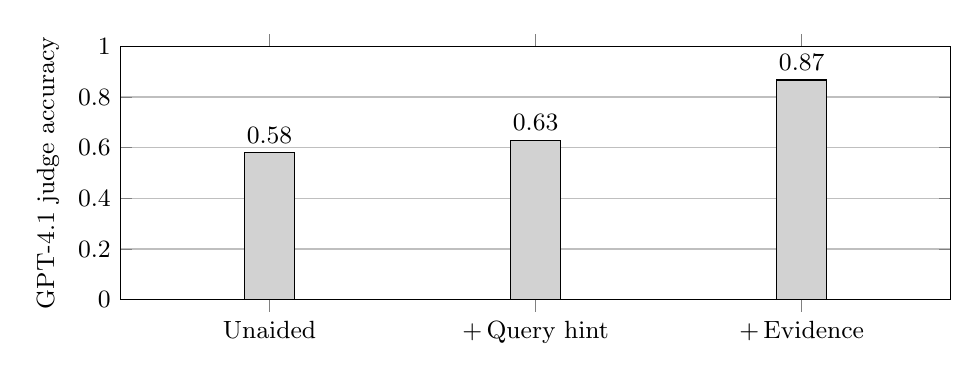
\begin{tikzpicture}
\begin{axis}[
    ybar,
    width=\columnwidth,
    height=4.8cm,
    bar width=18pt,
    ymin=0, ymax=1,
    ylabel={GPT-4.1 judge accuracy},
    xtick={1,2,3},
    xticklabels={Unaided, {+\,Query hint}, {+\,Evidence}},
    enlarge x limits=0.28,
    ymajorgrids,
    nodes near coords,
    every node near coord/.append style={font=\small,
        /pgf/number format/fixed, /pgf/number format/precision=2,
        /pgf/number format/fixed zerofill},
    tick label style={font=\small},
    label style={font=\small},
]
\addplot[fill=gray!35] coordinates {(1,0.5797) (2,0.6294) (3,0.8668)};
\end{axis}
\end{tikzpicture}
\caption{LoRA r16 on the $398$ judge-approved teacher rows. A teacher query-string hint barely lifts judge accuracy over the unaided adapter, whereas supplying the teacher's retrieved evidence accounts for nearly all of the recovery---the binding constraint is acquiring evidence, not generating answers. Values match Table~\ref{tab:queryhint}.}
\label{fig:gap}
\end{figure}

\subsection{Query-Only LoRA and Deterministic Query Skeletons}

Query-only LoRA uses only \tool{conversation\_search} targets. Token-level metrics are strong, but the adapter fails as an end-to-end agent because it cannot reliably preserve tool calls in the correct channel or transition from search to answer. A deterministic query skeleton removes these burdens: the model emits only a query string and a wrapper supplies the tool shell.

\begin{table}[t]
\centering
\small
\begin{tabular}{lrrr}
\toprule
\textbf{Query generator} & \textbf{Rows} & \textbf{Ret-ref} & \textbf{Cont.} \\
\midrule
Query-only, phase-routed & 100 & 0.09 & 0.11 \\
Query-only, skeleton & 100 & 0.23 & 0.23 \\
Full r16, skeleton & 100 & 0.16 & 0.17 \\
\bottomrule
\end{tabular}
\caption{Deterministic skeleton reveals useful query signal hidden by tool-call shell failures.}
\label{tab:skeleton}
\end{table}

On the 500-row raw split, the query-only skeleton reaches retrieved-reference $0.244$ and containment $0.216$. That the same adapter does so much better once stripped of the tool-call shell tells us the query signal was there all along, hidden by the agent interface.

\subsection{Teacher Query Replay Quantifies the Remaining Gap}

Replaying GPT-4.1's own query strings in the same deterministic skeleton sets an upper reference. Both the full teacher chains and the budget-matched max-3 chains retrieve better than the student's query-only skeleton.

\begin{table*}[t]
\centering
\small
\begin{tabular}{llrrrr}
\toprule
\textbf{Condition} & \textbf{Subset} & \textbf{Rows} & \textbf{Ret-ref} & \textbf{Cont.} & \textbf{Mean retrieved} \\
\midrule
Teacher full chain & approved & 398 & 0.442 & 0.405 & 4.36 \\
Teacher full chain & teacher-search & 302 & 0.583 & 0.533 & 5.74 \\
Teacher max-3 & approved & 398 & 0.367 & 0.342 & 3.25 \\
Teacher max-3 & teacher-search & 302 & 0.483 & 0.450 & 4.28 \\
Query-only skeleton & approved & 398 & 0.276 & 0.249 & 3.76 \\
Query-only skeleton & teacher-search & 302 & 0.272 & 0.238 & 3.76 \\
\bottomrule
\end{tabular}
\caption{Teacher query replay in the deterministic skeleton. The student remains far below teacher query quality.}
\label{tab:teacherquery}
\end{table*}

The row-level gap on the teacher-search subset is lopsided: $72/302$ rows are retrieved by the teacher's query alone against only $8/302$ by the student's. Three patterns recur in the student's misses---copying the probe phrasing verbatim, reaching for a plausible but wrong answer prior, and omitting the discriminative literal that would have anchored the search.

\subsection{Hard-Set SFT and DPO Do Not Generalize}

We construct a teacher-only hard set of 72 rows where teacher max-3 retrieves the reference but query-only skeleton does not. Positive SFT and zero-result DPO recover a few hard rows but hurt the raw distribution.

\begin{table}[t]
\centering
\small
\resizebox{\columnwidth}{!}{%
\begin{tabular}{lrrrr}
\toprule
\textbf{Query generator} & \textbf{Raw ret.} & \textbf{Raw cont.} & \textbf{Hard ret.} & \textbf{Hard cont.} \\
\midrule
Query-only skeleton & 0.244 & 0.216 & 0/72 & 1/72 \\
Hard-positive SFT & 0.184 & 0.180 & 7/72 & 7/72 \\
Preference zero-DPO & 0.166 & 0.158 & 8/72 & 7/72 \\
\bottomrule
\end{tabular}%
}
\caption{Small hard-set SFT/DPO recovers some hard rows but does not generalize.}
\label{tab:hard}
\end{table}

\subsection{Candidate Query Reranking Improves Hard Failures}

We next generate multiple candidate queries at each search step and rerank them using non-oracle local retrieval feedback. The lexical reranker scores result count, query specificity, probe/evidence overlap, repeated-query penalties, broad-result penalties, and repeated-evidence penalties. It never uses the reference answer.

\begin{table}[t]
\centering
\small
\begin{tabular}{lrrr}
\toprule
\textbf{Query strategy} & \textbf{Ret-ref} & \textbf{Cont.} & \textbf{Mean ret.} \\
\midrule
Query-only skeleton & 0.244 & 0.216 & 3.744 \\
Hard-positive SFT & 0.184 & 0.180 & 2.882 \\
Preference zero-DPO & 0.166 & 0.158 & 2.564 \\
Count rerank, target 3 & 0.210 & 0.202 & 3.218 \\
Lexical rerank, target 5 & 0.246 & 0.224 & 4.742 \\
\bottomrule
\end{tabular}
\caption{Raw500 query-policy results. Lexical reranking is the first non-oracle setting that slightly improves the full distribution.}
\label{tab:rerankraw}
\end{table}

On the teacher-only hard 72 rows, lexical reranking retrieves the reference in $25/72$ rows and raises containment to $22/72$, far above SFT/DPO pilots.

\subsection{Evidence Filtering Reduces Context Volume}

Candidate lexical reranking increases retrieval volume, creating more distractors for the answer model. We therefore apply a final non-oracle lexical evidence filter before answer generation.

\begin{table}[t]
\centering
\small
\begin{tabular}{lrrr}
\toprule
\textbf{Condition} & \textbf{Ret-ref} & \textbf{Cont.} & \textbf{Mean ret.} \\
\midrule
Query-only skeleton & 0.244 & 0.216 & 3.744 \\
Lexical rerank & 0.246 & 0.224 & 4.742 \\
Rerank + filter top-6 & 0.234 & 0.224 & 3.426 \\
\bottomrule
\end{tabular}
\caption{Evidence filtering preserves containment while reducing retrieved evidence volume.}
\label{tab:filter}
\end{table}

Filtering slightly reduces retrieved-reference but preserves final containment. On hard72, retrieved-reference decreases from $25/72$ to $23/72$, while containment remains $22/72$. On zero51, retrieved-reference decreases from $18/51$ to $16/51$, while containment remains $15/51$. This result is best read as a context-efficiency gain rather than a new accuracy gain: query-time recall and answer-time context size can be optimized separately.

\section{Discussion}

\paragraph{The bottleneck is evidence acquisition, not answer generation.}
The same pattern surfaces across conditions. Full-history prompting more than doubles strict-template containment; teacher-trace replay lets frozen students answer most rows; and on the approved subset the r16 adapter climbs from $0.5797$ unaided to $0.8668$ once teacher evidence is supplied. The model can usually answer when the evidence is in front of it---what it cannot do reliably is retrieve that evidence itself. Query selection is a large part of this: replayed deterministically, the teacher's queries recover answer-bearing memory far more often than the student's ($0.483$ versus $0.272$ on the searched subset). But hinting those queries inside the agent loop barely moves the result ($0.5797 \to 0.6294$), because the student neither adopts them reliably nor consistently grounds what it retrieves.

\paragraph{Tool use and query selection are different problems.}
Strict-template repair and LoRA distillation buy loop completion but not retrieval accuracy. Query-only LoRA fails the other way: it learns serviceable query strings yet cannot hold together as a full agent. A single adapter should not be asked to handle tool-call transport, query selection, phase transition, and answer generation at once.

\paragraph{Teacher trajectories help but must be audited.}
GPT-4.1 is a strong teacher, yet its trajectories mix clean paraphrases with no-search answers, memory patches, and leniently judged rows. Treating them as gold would overstate our claims and contaminate query-policy training; the safer framing is judge-filtered supervision, with stricter subsets reserved for query-specific objectives.

\paragraph{Search-time control beats small hard-set fine-tuning.}
Hard-positive SFT and zero-result DPO memorize a few hard rows at the cost of raw performance. Candidate reranking instead uses the retriever as feedback at inference time: the model proposes several imperfect queries and the controller keeps the one whose local results look most useful. This targets the failure more directly, and it is the only non-oracle setting that improves the full distribution without a training run.

\section{Limitations}

Our setup is a local substring recall path, not the full MemGPT retrieval stack, and GPT-4.1 is not the model used in the original MemGPT experiments. The strict-template baseline predates the explicit substring contract that the teacher and LoRA runs adopt, so it anchors the diagnostic ladder but is not a fully controlled comparison point; the contained subset comparisons (Tables~\ref{tab:teacherablation} and~\ref{tab:queryhint}) are the controlled ones. The teacher traces are judge-filtered supervision rather than gold trajectories, and GPT-4.1 judging is no substitute for human evaluation. Fine-tuning is confined to Llama-3-8B; Mistral-7B serves only as a frozen replay diagnostic. The reranker and evidence filter are lexical heuristics, and the hard-set SFT/DPO pilots are small, so the negative preference-learning result is a diagnostic finding in this setting, not a general claim about DPO for memory-query optimization.

\section{Reproducibility and Ethical Considerations}

All experimental claims are tied to local artifacts under \tool{docs/}, \tool{data/evaluation/}, \tool{data/trajectories/}, and \tool{outputs/}. The DMR recall contract, model checkpoints, LoRA adapters, teacher filtering, and reranking/evidence-filtering diagnostics are documented in the corresponding reports. The most important reproducibility caveat is that teacher collection uses a fixed GPT-4.1 snapshot and a local substring memory contract.

The experiments use conversational memory data from a benchmark derived from multi-session chat. This setting is privacy-sensitive by nature, even when benchmark data are synthetic or anonymized. A memory agent that retrieves personal facts must avoid exposing unrelated private details and must distinguish evidence-grounded answers from guesses.

\section{Conclusion}

Small open-source LLMs can imitate parts of MemGPT-style memory behavior, but robust long-term retrieval does not fall out of trajectory distillation alone. The failures arrive in sequence. Raw models miss the tool-call contract; strict formatting repairs the surface but leaves retrieval weak; teacher-trace replay shows the models can usually answer once evidence is present; and LoRA distillation stabilizes the loop and the answering step while the full agent stays bottlenecked on the evidence it must retrieve for itself---query selection chief among the missing pieces.

The broader implication is that small memory agents should be built and evaluated as modular systems. Tool-call channel control, query selection, retrieval-feedback reranking, evidence filtering, and answer grounding are distinct capabilities, and copying them wholesale from a single teacher trajectory is too coarse a target. Future work should train and measure these components separately, and place query-policy diagnostics ahead of broad claims about long-term memory ability.

\bibliography{references}

\appendix
\section{Artifact Map}

\begin{table*}[t]
\centering
\small
\begin{tabularx}{\textwidth}{ll}
\toprule
\textbf{Component} & \textbf{Artifact} \\
\midrule
Vanilla and strict-template baseline & \tool{docs/experiment\_1\_report.md} \\
DMR protocol & \tool{docs/vanilla\_dmr\_protocol.md} \\
Teacher trajectory and replay & \tool{docs/oracle\_experiment\_report.md} \\
Teacher quality audit & \tool{docs/teacher\_containment\_mismatch\_audit.md} \\
LoRA training & \tool{docs/lora\_training.md} \\
Post-LoRA evaluation & \tool{docs/post\_lora\_evaluation\_report.md} \\
Failure audit & \tool{docs/failure\_audit\_report.md} \\
Teacher evidence ablation & \tool{docs/teacher\_evidence\_ablation\_report.md} \\
Teacher query hint & \tool{docs/teacher\_query\_ablation\_report.md} \\
Query-only LoRA & \tool{docs/query\_only\_lora\_report.md} \\
Deterministic query skeleton & \tool{docs/query\_skeleton\_dmr\_report.md} \\
Teacher query replay & \tool{docs/teacher\_query\_skeleton\_report.md} \\
Query gap analysis & \tool{docs/query\_skeleton\_gap\_report.md} \\
Hard-positive SFT & \tool{docs/query\_hard\_positive\_lora\_report.md} \\
Zero-result DPO & \tool{docs/query\_preference\_dpo\_report.md} \\
Candidate reranking & \tool{docs/query\_candidate\_rerank\_report.md} \\
Evidence filtering & \tool{docs/evidence\_filter\_report.md} \\
\bottomrule
\end{tabularx}
\caption{Local artifacts supporting each claim.}
\label{tab:artifacts}
\end{table*}

\section{Main Result Summary}

\begin{table*}[t]
\centering
\small
\begin{tabular}{llrrrr}
\toprule
\textbf{Condition} & \textbf{Model} & \textbf{Rows} & \textbf{Loop} & \textbf{Cont.} & \textbf{Judge} \\
\midrule
Raw vanilla pilot & Llama-3-8B & 5 & 0/5 & -- & -- \\
Strict-template DMR & Llama-3-8B & 500 & 481/500 & 0.1954 & -- \\
Full-history & Llama-3-8B & 500 & 500/500 & 0.5080 & -- \\
Full-history & Mistral-7B & 500 & 500/500 & 0.4240 & -- \\
Teacher-trace replay & Llama-3-8B & 398 & 398/398 & 0.4246 & 0.7337 \\
Teacher-trace replay & Mistral-7B & 398 & 398/398 & 0.4598 & 0.8769 \\
LoRA r8 end-to-end & Llama-3-8B & 500 & 489/500 & 0.2474 & 0.4765 \\
LoRA r16 end-to-end & Llama-3-8B & 500 & 497/500 & 0.2656 & 0.4809 \\
LoRA r16 + teacher query hint & Llama-3-8B & 398 & 394 comp. & 0.3452 & 0.6294 \\
LoRA r16 + teacher trace & Llama-3-8B & 398 & -- & 0.4899 & 0.8668 \\
\bottomrule
\end{tabular}
\caption{End-to-end and replay conditions. End-to-end rows are scored on the full set; the teacher-query-hint and teacher-trace rows cover the $398$ judge-approved subset, whose matched unaided baselines appear in Tables~\ref{tab:teacherablation} and~\ref{tab:queryhint}.}
\label{tab:mainappendix}
\end{table*}

\section{Representative Query Behavior}
\label{app:examples}

Table~\ref{tab:examples} contrasts teacher and student search queries on rows where the teacher's deterministic skeleton retrieves the reference-bearing utterance but the student's does not. Three patterns recur. The student copies long probe phrases that never appear verbatim in memory (row~33). It reaches for a plausible but wrong answer prior and searches for that instead---on row~5, \emph{dogs} crowds out the correct \emph{cat}, and the student then answers ``I have a dog.'' Or it issues the right broad terms but never narrows to the discriminative literal (rows~10 and~65, where the answer ends in \tool{UNKNOWN}).

\begin{table*}[t]
\centering
\small
\begin{tabularx}{\textwidth}{l l X X l}
\toprule
\textbf{Row} & \textbf{Reference} & \textbf{Teacher queries} & \textbf{Student queries} & \textbf{Pattern} \\
\midrule
33 & California! & studio, California, Santa Barbara & audio studio, audio studio location, your audio studio & probe-phrase copying \\
5 & I have a cat. & pets, cat, cats & pet, dogs, dogs & wrong answer prior \\
10 & Construction, like my dad. & job, work, construction & living, jobs, work & missing literal \\
65 & The Navy! & military, Navy & military service, branch, army & missing literal \\
\bottomrule
\end{tabularx}
\caption{Teacher-only retrieval rows from the deterministic query skeleton: the teacher's \tool{conversation\_search} strings retrieve the reference-bearing memory while the student's do not. Queries are listed in search order.}
\label{tab:examples}
\end{table*}

When the student does succeed, it is usually because a literal anchor from the probe survives into memory. On row~3 the chain \emph{part-time job}, \emph{McDonald's}, \emph{working at} pulls back the utterance behind the reference \emph{Burger King!}---even though the model never types ``Burger King''---and on row~96 \emph{taco}, \emph{fish tacos}, \emph{fish} recovers \emph{Fish tacos with cilantro lime slaw}. The failures above are thus not erratic search behavior but a consistent shortfall in choosing discriminative literal queries, which the candidate reranker (Table~\ref{tab:rerankraw}) targets at inference time.

\end{document}
